\section{Experiments}
\label{sec:experiment}

%\begin{table*}[th!]
%	\centering
%	\scriptsize
%	\begin{tabular}{l|llcc}
%		\toprule
%		\textbf{Dataset} &\textbf{Premise}  & \textbf{Choices} & \textbf{Training size} & \textbf{Test size}\\
%		\midrule
%		\multirow{4}{*}{ROC} & Sarah was home alone. &\multirow{2}{*}{Sarah then happily watched the show.     %\checksymbol}&\multirow{4}{*}{1871}&\multirow{4}{*}{1871}\\
%						&She wanted to stay busy. & 	\multirow{2}{*}{Sarah could not find anything to watch. \crosssymbol } \\
%						&She turned on the TV. \\
%						&She found a reality show to watch.\\
%		\midrule
%		\multirow{3}{*}{ARCT} &\textbf{Reason}: Milk isn’t a gateway drug even though &\textbf{Warrant 1}: Milk is similar to marijuana. \checksymbol&\multirow{3}{*}{1210}&\multirow{3}{*}{444}\\
%		&most people drink it as children. &\textbf{Warrant 2}: Milk is not marijuana.\crosssymbol \\
%		&\textbf{Claim}: Marijuana is not a gateway drug. \\
%		\midrule
%		\multirow{4}{*}{RECLOR} &\textbf{Context}:In a business...to financial prosperity. &A: ignores the fact that in... the family 's prosperity.\checksymbol&\multirow{4}{*}{4638}&\multirow{4}{*}{500}\\
%		&\textbf{Question}:The reasoning in the argument&B: presumes, without... the family's prosperity.\crosssymbol&\\
%		& is flawed because the argument&C: ignores the fact... even if they pay high wages.\crosssymbol\\
%		&&D: presumes, without providing...can succeed.\crosssymbol\\
		
		
%		\bottomrule
%	\end{tabular}
%	\caption{Examples for three datasets. The right choice is labeled with \checksymbol, the wrong choice is labeled with  \crosssymbol .}
%	\label{table:dataset}
%\end{table*}

\begin{table*}[th!]
	\centering
	\scriptsize
	\begin{tabular}{l|lccc}
		\toprule
		\textbf{Dataset} &\textbf{Premise}  & \textbf{Choices} & \textbf{Training size} & \textbf{Test size}\\
		\midrule
		\makecell[c]{COPA} &  \makecell[l]{The man hurt his back.} &\makecell[l]{He stayed in bed for several days.     \checksymbol 
		\\He went to see a psychiatrist. \crosssymbol }&\makecell[c]{500}&\makecell[c]{500}\\
		\midrule
		\makecell[c]{ROC} &  \makecell[l]{Sarah was home alone.\\She wanted to stay busy.\\She turned on the TV.\\She found a reality show to watch.} &\makecell[l]{Sarah then happily watched the show.     \checksymbol 
		\\Sarah could not find anything to watch. \crosssymbol }&\makecell[c]{1871}&\makecell[c]{1871}\\
		\midrule
		\makecell[c]{ARCT} &\makecell[l]{\textbf{Reason}: Milk isn’t a gateway drug even though \\ most people drink it as children. \\\textbf{Claim}: Marijuana is not a gateway drug.}&\makecell[l]{\textbf{Warrant 1}: Milk is similar to marijuana. \checksymbol \\
		\textbf{Warrant 2}: Milk is not marijuana.\crosssymbol}&\makecell[c]{1210}&\makecell[c]{444}\\
		\midrule
		\makecell[c]{RECLOR} &\makecell[l]{\textbf{Context}:In a business...to financial prosperity. \\
		\textbf{Question}:The reasoning in the argument\\  is flawed because the argument}&\makecell[l]{A: ignores the fact that in... the family 's prosperity.\checksymbol
		\\B: presumes, without... the family's prosperity.\crosssymbol
		\\C: ignores the fact... even if they pay high wages.\crosssymbol
		\\D: presumes, without providing...can succeed.\crosssymbol}&\makecell[c]{4638}&\makecell[c]{500}\\
		
		
		\bottomrule
	\end{tabular}
	\caption{Examples for all 4 datasets considered in this paper.}
	\label{table:dataset}
\end{table*}

%1. Re-evaluate the extent to which the model is exploiting short circuit after augmentation. Test it on the same sampled examples to see the improvement of percentage of cases where model look at context.


First, we show the experimental setup. 
Second, we compare several operators for testing short circuit problem and apply the best one to multiple models on diverse NL reasoning tasks.
Third, we evaluate the robustness of models with different augmentation methods.

\subsection{Experimental Setup} 
\label{sec:setup}
In this section, we will show our setup for datasets, models and test operators.
\subsubsection{Datasets}
We experiment on 4 datasets from four different tasks:
%\KZ{I think you need to say what is the context and what are the
%choices for these four datasets.}

\textbf{ROC} is a story ending prediction dataset. 
The task is to identify the correct ending of a four-sentence 
story premsie from two alternative choices. 

\textbf{COPA} is a causal reasoning dataset, an example is previously shown
in~\secref{sec:intro}. Given a premise, 
COPA requires choosing the more plausible, causally related choice. 
%There are 500 instances in 
%training data and 500 instances for testing.

\textbf{ARCT} is an argument reasoning comprehension dataset. 
There may exist an alternative warrant choice 
in which the reason is connected to the claim.

\textbf{RECLOR} is a reading comprehension dataset which requires logical reasoning.

Examples and statistics of these datasets are shown in~\tabref{table:dataset}. 

\subsubsection{Models}
We mainly investigate three popular classifiers based on pre-trained language models. 
There are several available versions of pre-trained models differing in the number of layers and parameters. We choose to use base version of each model. We train and test all the models on a server: a GeForce GTX 1080 Ti GPU with 11G RAM and Intel(R) Xeon(R) CPU E5-2630 with 128G of RAM.

\textbf{BERT} (BT) is a popular attention model, which applies the bidirectional training of Transformer. 
%The basic one has 12-layer transformer, blocks, 768 hidden-size, and 12 self attention, 
%heads, totally 110M parameters and fine-tune for 3 epochs to predict the relation based on context and 
%choices.

\textbf{XLNet} (XL) is trained with Permutation Language Modeling and without NSP.

\textbf{RoBERTa} (RB) is an improved pre-training procedure of BERT.

Besides the original models (marked as w/o), we also train these three
models with four competing data augmentation methods: 
back-translation~\cite{back2019} (B),  crossover (C), mutation (M)
and crossover + mutation (C+M). 
%The expanded data volume for each augmentation method are all consistent with the original data volume.
The expanded data volume is equal to the original data volume and 
the size of new train dataset has doubled.

\subsubsection{Stress Test Cases}
Following previous research~\cite{checklist2020acl}, 
we will test the effectiveness of different data augmentation
methods by looking at the robustness of models against
different stress tests.
We create these stress test cases using the proxy operations
introduced in \tabref{table:proxyop}.
Different operations generate different number of cases 
as shown in \tabref{tab:cases}. To evaluate the
ability of testing for short-circuiting, we will
use a subset of these test cases whose original MCQs are correctly answered by models in the next section.
%negation-add(Neg+),  negation-remove(Neg-), 
%NER, pronoun-replacement(PR), pronoun-instantiation(PI), 
%crossover(CO), adverbial(Adv), mutation(MT), Voice and synonym(Syn). 

\begin{table}[th]
\centering
\scriptsize
\begin{tabular}{c|rrrr}
\toprule
\textbf{Stress} & \textbf{ROC} & \textbf{COPA} & \textbf{ARCT} & \textbf{RECLOR} \\ \midrule
Neg+  &	1,797&492&	297&375	\\ \hline
Neg-  &	94&	2&	152&	119\\ \hline
NER  &	362&	0&	5&0	\\ \hline
PR  &	1,073&	328&71&72	\\ \hline
PI  &	     861&	219&	56&	91\\ \midrule
Adv  &	1,850&496	&444	&500	\\ \hline
CO  &	1,871&500	&444	&500	\\ \hline
Syn&	653&	 25&	303&289	\\ \midrule
MT  &	1,871&500	&444	&500	\\ \hline
Voice  &	1,014&246	&174	&263	\\ \hline
Total & 11,446  &  2,808 & 2,390 & 2,709 \\ \bottomrule
\end{tabular}
\caption{Number of stress test cases \protect\footnotemark generated
by different operations for 4 datasets.}
\label{tab:cases}
\end{table}

\footnotetext{The number denotes the number of questions 
which can be transfered to a new stress test case with a certain operation.}
%we divide the stress test into two parts, the above part of~\tabref{table:tripleclassification} 
%are test types without syntax and  semantic errors, the following are test cases with errors.  
%compare different we re-evaluate the 
%exploiting short give the results
%on cue discovery as well as model probing along with some analysis. The whole framework has been implemented into
%an online demo at 
%review.

\subsection{Testing for Short Circuit}
\label{sec:short_circuit}
In this section, we will select proper testing operators for short circuit testing and 
we use these operators to detect the extent of model short circuit.

\subsubsection{Selecting Short Circuit Testing Methods}
\label{sec:select-sc}
%\KZ{Here we evaluate different black-box tests available to
%detect short-circuits in 3 different models. The ground truth
%is the attention map results generated by roy's code.}
%In~\secref{sec:proxy}, we have discussed the possibility that both white-box attention-based method and black-box choice operators 
%in some of the equivalent classes can evaluate short circuits. 
We now evaluate which proxy test operators are better suited for short circuit evaluation.
%For further exploring which operator is better for short circuit evaluation, 
%we sampled 100 random ROC questions that models had already done right for human annotation labeling. 
%Human annotators were asked to determine whether the model considered both premise and choice at the same time 
%with a visual attention map tool. 
%Different with AW,  human annotators are capable of reasoning, 
%and they do not consider relationships that have nothing to do with the answer, 
%such as punctuation and stop words between premise and choices. 
%As described in \secref{sec:proxy}, 
Each test operator generates new test cases by making directional changes to
the test cases that the model answers correctly. 
The model is considered not short-circuiting on a case according 
to a test operator if it still gets the right answer after the operation. 
%Assuming that human attention annotation, attention weight thresholding (AW), 
%and each choice operator are all plausible proxy tests, 

Including human attention annotation and choice-only test, we compare 8 different 
proxy tests in \tabref{tab:agree}. 
%In AW, the hyper parameter $t_1$ and $t_2$ are tuned to 0.14 and 0.13 separately 
We randomly sample 30 MCQs from the test set of ROC that are correctly answered 
by three models respectively. 
For each proxy test, we constructed a binary proxy vector 
of 30-dimensional one-hot vector~(proxy vector) for each model, where each dimension refers to 
a test case passing that proxy test (1) or not (0). If a model doesn't pass the proxy test 
on a certain test case, it means that model short-circuits on that specific MCQ. 
If a test case is not applicable to a proxy test, we generate 0 or 1 randomly.
%Each proxy test will produce a 30-dimensional one-hot vector~(proxy vector) for each model, where 1/0 indicates if the 
%model short-circuited on that specific MCQ or not. 
%\footnote{For MCQ where a certain proxy test is not applicable, we 
%randomly label it as 1 or 0.}. 
For each model, we then compute another vector as the ensemble of all proxy tests by 
majority voting on each of the 30 dimensions. We use the Euclidean distance between the 
proxy vector and the ensemble vector (i.e., center) because the test 
closest to the center will be the most 
representative and applicable to most test cases.  
%The smaller euclidean distance between the individual proxy vector of each test type 
%and the ensemble vector indicates higher reliability. 
We can find that the results of CO are generally closer to the ensembled results. 
Thus, we use CO as the proxy test for short circuit evaluation in the rest of
this section. 

\begin{table}[t]
	\scriptsize
	\centering
	\begin{tabular}{c|cccc}\hline
		\toprule  
		\textbf{Test types} &BERT  & XLNet & RoBERTa  &Ave\\ 
		\midrule
		{Neg+}      &  4.24   	&   3.46  &	\textbf{2.65}	&3.45\\
		\midrule
		{Neg-}&   4.0 	&       3.61  &	3.87	&3.83\\
		\midrule
		{NER}    &   4.0 	&  3.46      &	4.24	&3.9\\
		\midrule
		{PR}&    4.0 	&    3.32   &	4.0	&3.77\\
		\midrule
		{PI}&   3.32 	&    4.0    &	3.16	&3.49\\
		\midrule
		{CO}  &      \textbf{2.0}   	&  \textbf{ 2.0} &	2.83	&\textbf{2.28}\\
		\midrule
		%{AW}   &  \textbf{2.45}	&3.46&	\textbf{2.45}	&\textbf{2.79} \\
		%\midrule
		{Choice-only}   &  4.12  	&3.87  &	3.87	&3.95\\
		\midrule
		{Human}   & 2.24	&   3.0&	3.0	&2.75\\
		\bottomrule
		\hline
	\end{tabular}
	\caption{\label{tab:agree} 
		Euclidean distances between proxy vector and 
		the ensemble vector on short circuit test (the smaller
		the better). 
		Ave is the average score across all models.
		Top test type for each model are highlighted.}
\end{table}

\begin{table*}[t!]
	\scriptsize
	\centering
	\begin{subtable}[t]{0.48\textwidth}
		\centering
		\begin{tabular}{l|c|cc}\toprule
			\multirow{2}{*}{\textbf{Model}}& \multirow{2}{*}{\bf Short circuit Tests} & \multicolumn{2}{c}{\bf Robustness Tests} \\ \cline{3-4}
			& & \textbf{Original} &\textbf{Stress}\\ \hline
			\rowcolor{Gray}
			BT(w/o)&90.80&86.58&81.93\\
			BT+B&92.54&86.75&82.96\\
			BT+C&\textbf{98.47}&\textbf{87.07}&84.34\\
			BT+M&91.47&86.48&86.06\\
			BT+C+M&97.78&86.75&\textbf{88.60}\\
			\midrule
			
			\rowcolor{Gray}
			XL(w/o)&83.28&\textbf{90.81}&79.22\\
			XL+B&84.4&90.43&82.23\\
			XL+C&\textbf{98.81}&89.47&86.23\\
			XL+M&86.90&90.17&89.47\\
			XL+C+M&97.10&90.22&\textbf{92.64}\\
			\midrule
			\rowcolor{Gray}
			RB(w/o)&88.76&\textbf{92.73}&82.33\\
			RB+B&87.98&92.46&78.50\\
			RB+C&\textbf{99.3}&91.18&88.92\\
			RB+M&88.06&92.62&90.29\\
			RB+C+M&97.44&91.88&\textbf{93.06}\\
			\bottomrule
		\end{tabular}
		\caption{ROC}
	\end{subtable} 
	\hfill
	\begin{subtable}[t]{0.48\textwidth}
		\centering
		\begin{tabular}{l|c|cc}\toprule
			\multirow{2}{*}{\textbf{Model}}& \multirow{2}{*}{\bf Short circuit Tests} & \multicolumn{2}{c}{\bf Robustness Tests} \\ \cline{3-4}
			& & \textbf{Original} &\textbf{Stress}\\ \hline
			\rowcolor{Gray}
			BT(w/o)&68.71&62.00&57.40\\
			BT+B&85.42&68.60&68.95\\
			BT+C&\textbf{97.25}&\textbf{72.80}&78.84\\
			BT+M&90.62&70.40&79.62\\
			BT+C+M&96.13&72.40&\textbf{80.68}\\
			\midrule
			
			\rowcolor{Gray}
			XL(w/o)&60.26&61.40&57.71\\
			XL+B&65.51&63.20&61.06\\
			XL+C&\textbf{94.69}&\textbf{67.80}&75.42\\
			XL+M&57.23&62.20&71.10\\
			XL+C+M&83.93&67.20&\textbf{81.32}\\
			
			\midrule
			
			\rowcolor{Gray}
			RB(w/o)&78.01&76.40&74.85\\
			RB+B&83.64&77.00&80.26\\
			RB+C&\textbf{98.23}&\textbf{79.00}&83.31\\
			RB+M&84.30&72.60&83.53\\
			RB+C+M&92.70&74.00&\textbf{87.30}\\
			\bottomrule
		\end{tabular}
		\caption{COPA}
	\end{subtable} 
	\hfill
	\begin{subtable}[t]{0.48\textwidth}
		\centering
		\begin{tabular}{l|c|cc}\toprule
			\multirow{2}{*}{\textbf{Model}}& \multirow{2}{*}{\bf Short circuit Tests} & \multicolumn{2}{c}{\bf Robustness Tests} \\ \cline{3-4}
			& & \textbf{Original} &\textbf{Stress}\\ \hline
			\rowcolor{Gray}
			BT(w/o)&78.52&63.96&58.08\\
			BT+B&61.18&68.47&56.21\\
			BT+C&\textbf{96.08}&\textbf{68.92}&65.73\\
			BT+M&74.42&67.79&69.65\\
			BT+C+M&90.0&67.57&\textbf{73.71}\\
			\midrule
			
			\rowcolor{Gray}
			XL(w/o)&59.10&75.45&61.72\\
			XL+B&60.40&\textbf{79.05}&64.78\\
			XL+C&\textbf{92.45}&74.55&69.93\\
			XL+M&59.57&74.10&73.15\\
			XL+C+M&90.35&77.03&\textbf{79.11}\\
			\midrule
			
			\rowcolor{Gray}
			RB(w/o)&60.29&78.83&66.16\\
			RB+B&60.94&\textbf{81.31}&66.02\\
			RB+C&92.77&77.93&70.64\\
			RB+M&68.13&77.03&76.64\\
			RB+C+M&\textbf{93.39}&75.00&\textbf{78.97}\\
			\bottomrule
		\end{tabular}
		\caption{ARCT}
	\end{subtable} 
	\hfill
	\begin{subtable}[t]{0.48\textwidth}
		\centering
		\begin{tabular}{l|c|cc}\toprule
			\multirow{2}{*}{\textbf{Model}}& \multirow{2}{*}{\bf Short circuit Tests} & \multicolumn{2}{c}{\bf Robustness Tests} \\ \cline{3-4}
			& & \textbf{Original} &\textbf{Stress}\\ \hline
			\rowcolor{Gray}
			BT(w/o)&50.88&45.60&33.91\\
			BT+B&61.73&\textbf{48.60}&35.99\\
			BT+C&\textbf{96.17}&47.00&47.72\\
			BT+M&58.55&46.80&50.02\\
			BT+C+M&87.16&43.60&\textbf{53.79}\\
			\midrule
			
			\rowcolor{Gray}
			XL(w/o)&62.86&56.00&39.77\\
			XL+B&74.04&\textbf{57.0}&44.6\\
			XL+C&\textbf{98.90}&54.40&51.66\\
			XL+M&70.15&53.60&56.99\\
			XL+C+M&88.56&54.2&\textbf{58.63}\\
			\midrule
			\rowcolor{Gray}
			RB(w/o)&70.2&51.00&36.76\\
			RB+B&73.73&51.00&38.71\\
			RB+C&\textbf{96.83}&50.40&50.88\\
			RB+M&80.38&\textbf{52.00}&\textbf{59.95}\\
			RB+C+M&88.43&48.40&55.78\\
			\bottomrule
		\end{tabular}
		\caption{RECLOR}
	\end{subtable}
	\caption{\label{tab:results} Short circuit and Robustness Tests
		on 4 models with or without(w/o) data augmentation.
		All numbers are percentages (\%). 
		+B = augmented with back-translation,
		+C = augmented with crossover, +M = augmented with mutation, 
		CO=crossover. 
		Stress includes all cases in \tabref{tab:cases}.}
	%Robustness Test includes: Neg+=negation-add, Neg-=negation-remove, NER, 
	%PR=pronoun-replacement, PI=Pronoun-instantiation, Adv=adverbial, MT=mutation, Voice, Syn=synonym.}
	
\end{table*}
It is noted that, we choose not to use a higher-dimensional vector
here because a) we are not computing accuracy or
pass rate, so statistical significance
is not an issue, and b) in a 30-dimensional space,
we can already sufficiently distinguish these short
circuit tests in \tabref{tab:agree}. Adding more test cases
or more dimensions will not change that distinction.

In our experiment, we do not use human labeling results on attention map 
as gold indicators.  Because the attention map on each model is not a direct 
expression of the final decision for multiple-choice questions, 
but the expression of the premise and choices which is an indirect information for reasoning.

%\begin{table}[th]
%\scriptsize
%\centering
%\begin{tabular}{c|cccc}\hline
%\toprule  
%\textbf{Test types} &BERT  & XLNet & RoBERTa  &Ave\\ 
% \midrule
%{Neg+}      &     30.06	 &46.67&	19.55	&32.09\\
%\midrule
%{Neg-}&    47.22	&63.33&	64.52	&58.36\\
%\midrule
%{NER}    &    49.94	&46.67	&51.61	&49.41\\
%\midrule
%{PR}&      30.99	&43.33	&38.71&	37.68\\
%\midrule
%{PI}&    34.07	&40&	35.48	&36.52 \\
%\midrule
%{CO}            &     21.98	&23.33	&25.81	&\textbf{23.71}\\
%\midrule
%{AW}   &     22.28	&40&	19.35&	\textbf{27.21}\\
%\midrule
%{choice-only}   &     22.28	&40&	19.35&	\textbf{27.21}\\
%\midrule
%{Human}   &75.98	&20	&29.03	&41.67\\
%\bottomrule
%\hline
%\end{tabular}
%\caption{\label{tab:agree} Euclidean distance between test type vector and the ensemble vector on short circuit test. Ave is 
%the average score across all models.}
%\end{table}






%Each operator in~\table{tab:agree} are possible to show whether the model has short circuit problem to a certain extent, In order to choose a more appropriate method, we adopt the following strategies: find the focus of these methods, that is, vote on a topic. If most methods think that the model cheats on this topic, then this topic will be considered cheating. According to the various methods and the Euclidean distance of the selected answer, choose the method that is more suitable for short-circuit test

%\begin{table}[th]
%\scriptsize
%\centering
%\begin{tabular}{c|ccc}\hline
%\toprule  
%\textbf{Test types} &BERT (\%) & XLNet (\%) & RoBERTa (\%)  \\ 
% \midrule
%{Neg+}      &     36.67      &      47.83   & 52  \\
%\midrule
%{Neg-}&     50     &   60 & 40  \\
%\midrule
%{NER}    &     66.67       &    42.85          &   35.71\\
%\midrule
%{PR}&      47.61       &    44.44      &  26.31  \\
%\midrule
%{PI}&     50           &   50    & 35.71  \\
%\midrule
%{CO}            &     83.33        & \textbf{ 70}       &    70.97\\
%\midrule
%{AW}   &      \textbf{99.6}     & 66.67 &   \textbf{77.42} \\
%\bottomrule
%\hline
%\end{tabular}
%\caption{\label{tab:agree} The agreement on short circuit 
%detection between human annotation and each proxy test.}
%\end{table}

\subsubsection{Testing Short Circuit Problems}
\label{sec:fix-sc}
%We test short circuits by observing AW and CO scores, 
%i.e., higher AW/CO scores indicate a lower chance for short-circuiting. We fine-tune the multiple choice classifiers of BERT, XLNet and RoBERTa on 4 datasets. 
Each number in ``Short Circuit Tests'' columns of
\tabref{tab:results} denotes
the percentage of test cases that pass 
the proxy short circuit test. 
The higher the percentage, the lower the possibility of short circuit problem.
Each group of models (e.g., BT*) are tested
on the subset of the original test set (1871 cases for ROC)
that vanilla model answers correctly.
For example, the test set for BT* on ROC contains 
1871*86.58\% = 1620 questions.

In~\tabref{tab:results}, we fine-tune the multiple-choice classifiers of BERT, XLNet and RoBERTa on 4 datasets 
with their original training data. 
We can find that all models trained on original data (in gray color) without 
data augmentation generally suffer from lower short-circuit passing rates. 
%We can find that the original models (the gray part in ``Short circuit Test'' column) without 
%data augmentation are most likely to have short-circuits because the CO score are quite low. 
%lower CO scores indicate a higher chance for short-circuiting. 
Unsurprisingly, all models tend to short-circuit on COPA, 
as it has been shown to contain easy-to-exploit 
single-token cues by prior work~\citep{kavumba-etal-2019-choosing}. 
RECLOR is a relatively hard task for models to solve as model 
accuracies on the original test set are generally 
lower than other tasks. 
Nevertheless, the fairly low short circuit test passing rates indicate that these models are still largely making use of superficial cues in the datasets. 
%Thus we can conclude that short circuit is a serious and common problem which is harmful for 
%model robustness on different tasks.

We further evaluate the augmented models (with white background in 
``Short Circuit Tests'' columns) 
using the short circuit test. According to \tabref{tab:results}, 
models augmented by crossover always gets the highest short circuit test
score. It indicates that model learns to reason jointly over both premise and choice. 
Back-translation doesn't help ameliorate short circuit much, 
possibly because cues being exploited are still kept after back-translation process. 
Mutation turns out to be not as effective as crossover for alleviating short circuit. 
This is likely due to mutation introducing incorrect syntax to the wrong choice, 
which makes it easier to be eliminated by models.



%\KZ{Remove the parts about overall robustness} 


%\begin{table}[th!]
%	\centering
%	\scriptsize
%	\begin{tabular}{ll|cc|cc}
%		\toprule
%		\textbf{Dataset} &\textbf{Model}  & \textbf{AW} & \textbf{CO\_sc} & \textbf{Original}&\textbf{Stress}\\
%		\midrule
%		\multirow{3}{*}{ROC} & BT &98.76&90.80&86.58&81.93\\
%		&XL& 28.08&83.28&90.81&79.22\\
%		&RB&77.41&88.76&92.73&82.33\\
%		\cmidrule{2-6}
%		\multirow{3}{*}{COPA} & BT &89.68&68.71&62.00&57.40 \\
%		&XL& 93.16&60.26&61.40&57.71\\
%		&RB&80.89&78.01&76.40&74.85\\ \cmidrule{2-6}
%		
%		\multirow{3}{*}{ARCT} & BT & 9.65&78.52&63.96&58.08\\
%		&XL& 85.67&59.10&75.45&61.72\\
%		&RB&  99.14&60.29&78.83&66.16\\ \cmidrule{2-6}
%			
%		\multirow{3}{*}{RECLOR} & BT &    82.46&50.88&45.6&33.91\\
%		&XL&  79.64&62.86&56.0&39.77\\
%		&RB&85.88&70.2&51.0&36.76\\
%		\bottomrule
%	\end{tabular}
%	\caption{Evaluation models with short circuit test and robustness 
%	test on 4 different datasets. $CO_sc$ denotes we use crossover operator for short circuit evaluation}
%	\label{tab:original}
%\end{table}


%\KZ{Compare crossover, mutation, backtranslation's abilities to
%fix the short-circuit problems. Use roy's code to evaluate
%the new models after augmentation to show that short-circuit problems
%drops the most under crossover.}

\subsection{Improving Overall Model Robustness}
In this subsection we test the model robustness against original test and 
stress test mentioned in \tabref{tab:cases}.
%with original training data and 
%different expanded training data.
\label{sec:robust}
%\KZ{Show that the models all vulnerable to different kinds of
%stress tests. And then how our data augmentation methods can
%improve the robustness of these models on 4 diff datasets.}


\subsubsection{Model Weakness}
%From previous work,  we have recognized the weakness of  
%models and the possible causes. 
%and are not robustness on stress test. 
%We fine-tune the multiple choice classifiers of on 4 datasets. 
Robustness test in~\tabref{tab:results} includes original test and stress 
test generated by all possible operators in \tabref{tab:cases}. 
The numbers in the ``Original'' columns denote the percentage of 
test cases correctly predicted by the models. 
For example, ROC has 1871 test cases~(\tabref{table:dataset}).
The scores in the ``Stress'' columns are the percentage of
stress test cases correctly predicted by the models.

In~\tabref{tab:results}, we can find that BERT, XLNet and RoBERTa models on different 
datasets are mostly not robust on stress test.
Compared with testing on original test data, 
the accuracy rate has dropped by 11.59\% for XLNet model trained with ROC. 
%Meanwhile, the AW short circuit score is 28.8\% which indicates this model may suffer from 
%short circuit. 
Similarly, all three models perform much 
worse than before on RECLOR and ARCT datasets by about 10\%. 
In most cases, the lower the short circuit passing rate, 
the lower the stress test accuracy of a model.
%which is consistent with the CO score (is also much lower than 100\%). 
From these experiments, we can conclude that the instability of the model is a common problem, 
and one of the most likely reasons is short circuit. 
%Mostly the AW and CO are consistent with each other, but 
%sometimes they are different on some baselines, like.... In fact, AW is white-box testing while CO is black-box testing. 
%Their behaviors are not intended to be the same.
%In practice, these two testing methods can complement 
%each other.
Due to limited space, we average the accuracies of different stress tests into a single number 
in the last column of \tabref{tab:results}. Please refer to the Appendix for complete results.


\subsubsection{Effects of Data Augmentation}
%\KZ{The weakness can be on the same table as the improvements
%to save space.}
%\KZ{Check the following analysis to make sure it's consistent with the tables.}
Compared with 
base models without data augmentation, we find that 
all four data augmentation methods moderately improve
the models when tested on the original test set. 
In ROC, accuracy of BERT and RoBERTa trained with crossover augmented data 
exceeds base models and ranks top. Crossover method also works on COPA. 
Even though back-translation obtains higher score mostly on ARCT and RECLOR,
crossover, mutation and crossover+mutation barely fall below the base model. 

Augmentation fares much better in the ``Stress'' columns, though
different methods show varying degree of success.
Compared with the model without data augmentation, 
the performance of models with crossover 
has always been greatly improved (i.e., by 21.44\% for BERT on COPA).
It indicates that reducing the short circuits 
is a good way to improve the robustness of a model.
%The performance of new models with crossover has 
%great improvement for all models on different dataset 
%compared with the model without data augmentation, like 21.44% for BERT on COPA. 
Mutation alone can also help with robustness on stress test better than crossover.
%This result suggests that mutation is a good method 
%for enhancing the robustness of models. 
Though, mutation may be not a 
good method to decrease the short circuits (\secref{sec:fix-sc}). 
Overall, crossover+mutation 
can mostly get the best performance on the stress test except for 
training on RECLOR with RoBERTa. 
%to This result indicates that this kind of data can prevent models from being confused 
%by simple perturbations thus improving the robustness of models. 
Besides, we can also find that back-translation doesn't improve the models' robustness much.
%Crossover alone can also help with robustness on stress test but 
%no better than mutation and crossover+mutation.  

%some of Table 5's AW scores being 
%some of Table 5's AW scores being 
%lower than AW for model w/o augmentation (e.g., 45.13 in (b)), 
%then the reason is AW is only a proxy test
%that catches majority of short circuit cases in our opinion, 
%but it's not perfect, as we pointed out in A2 of R1. 
%If you are referring to some accuracies in the Original columns 
%being lower than models w/o augmentation in Table 5 (e.g., 72.6 in (b)), 
%the reason is some models w/o augmentation might have 
%"cheated" to get high accuracy. Augmenting (C or M) corrects the
%biases in these models and may reduce the accuracy on the original test set.
%Nevertheless, all models after augmentation do better on the stress tests.

%have least short circuits based on BERT and XLNet. 
%Crossover+mutation based on RoBERTa takes less short circuits than others. 
%In the CO and AW columns, the result are consistent on ROC. 


\subsection{Case Study}
\label{sec:case}
To glean more insight on how our data augmentation methods help enhance model robustness on natural language reasoning, we perform case study by analyzing the change of attention patterns.

An example MCQ drawn from ROC test set is shown in \figref{fig:case_study} for
illustration. There is no positive attention value in front of the fourth sentence, so we intercept it from where it is worth. RoBERTa trained on the original training set fails to pick up the right choice likely due to there being virtually no attention connection between words in the choice and words in the premise. After training with crossover data augmentation, the model learns to build contextual reasoning  by attending to relevant concept in the premise, i.e., ``show'' in this example. The rationale behind such a change of attention pattern is that, in a MCQ created by crossover operation, the model needs to combine information in the premise to effectively distinguish the true ``right'' choice from the wrong one, which is also a right choice in another MCQ. Similar trends also exist for mutation operation as well as the combination of them. This observation empirically demonstrates the effectiveness of mitigating short circuit in terms of improving model robustness.  


\begin{figure}[th]
\centering
{\setlength{\fboxsep}{0pt}
\framebox{%
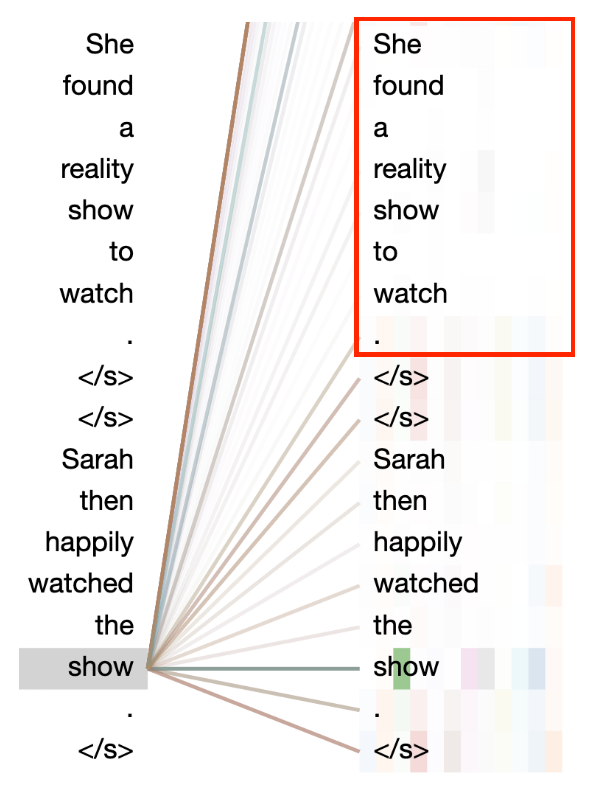
\includegraphics[width=0.47\columnwidth]{figure/o_un.eps}
}
\hfill
\framebox{%
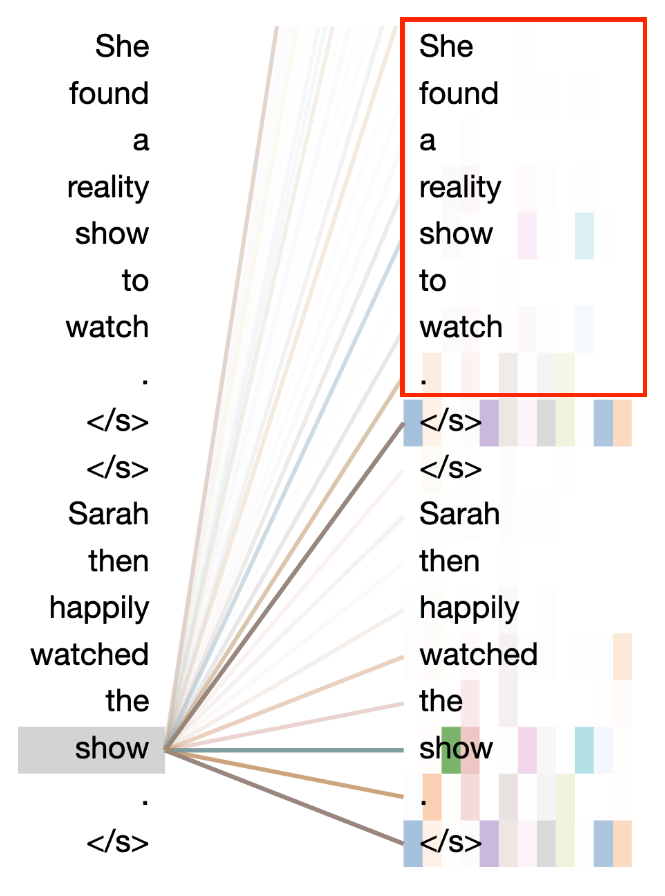
\includegraphics[width=0.47\columnwidth]{figure/cross_un.eps}
}
}
\caption{Attention maps showing that RoBERTa short-circuits on a ROC
question (left) and no longer short-circuits after data augmentation (right).}
\label{fig:case_study}
\end{figure}
